%	\section{Suite géométrique}
%	Les séries de termes suivants forment-ils une suite géométrique ? Donner le premier terme et la raison si c'est le cas.
%	\begin{questions}
%		
%	
%		\question[2] $\num{480} \: ; \: \num{-120} \: ; \: \num{30}  \: ; \:  \num{-7.5} \: ; \: \num{1.875}$ 
%		\fillwithdottedlines{3cm}
%		
%		\question[2] $\num{2} \: ; \:  \num{6} \: ; \: \num{18} \: ; \: \num{54} \: ; \: \num{162}$%152 
%		\fillwithdottedlines{3cm}
%		
%	\end{questions}
%	
	
\section{\'Equation de droite}

Dans le repère ci-dessous on a placé les points $A$ et $B$ et tracé la droite $(AB)$.


\begin{center}
	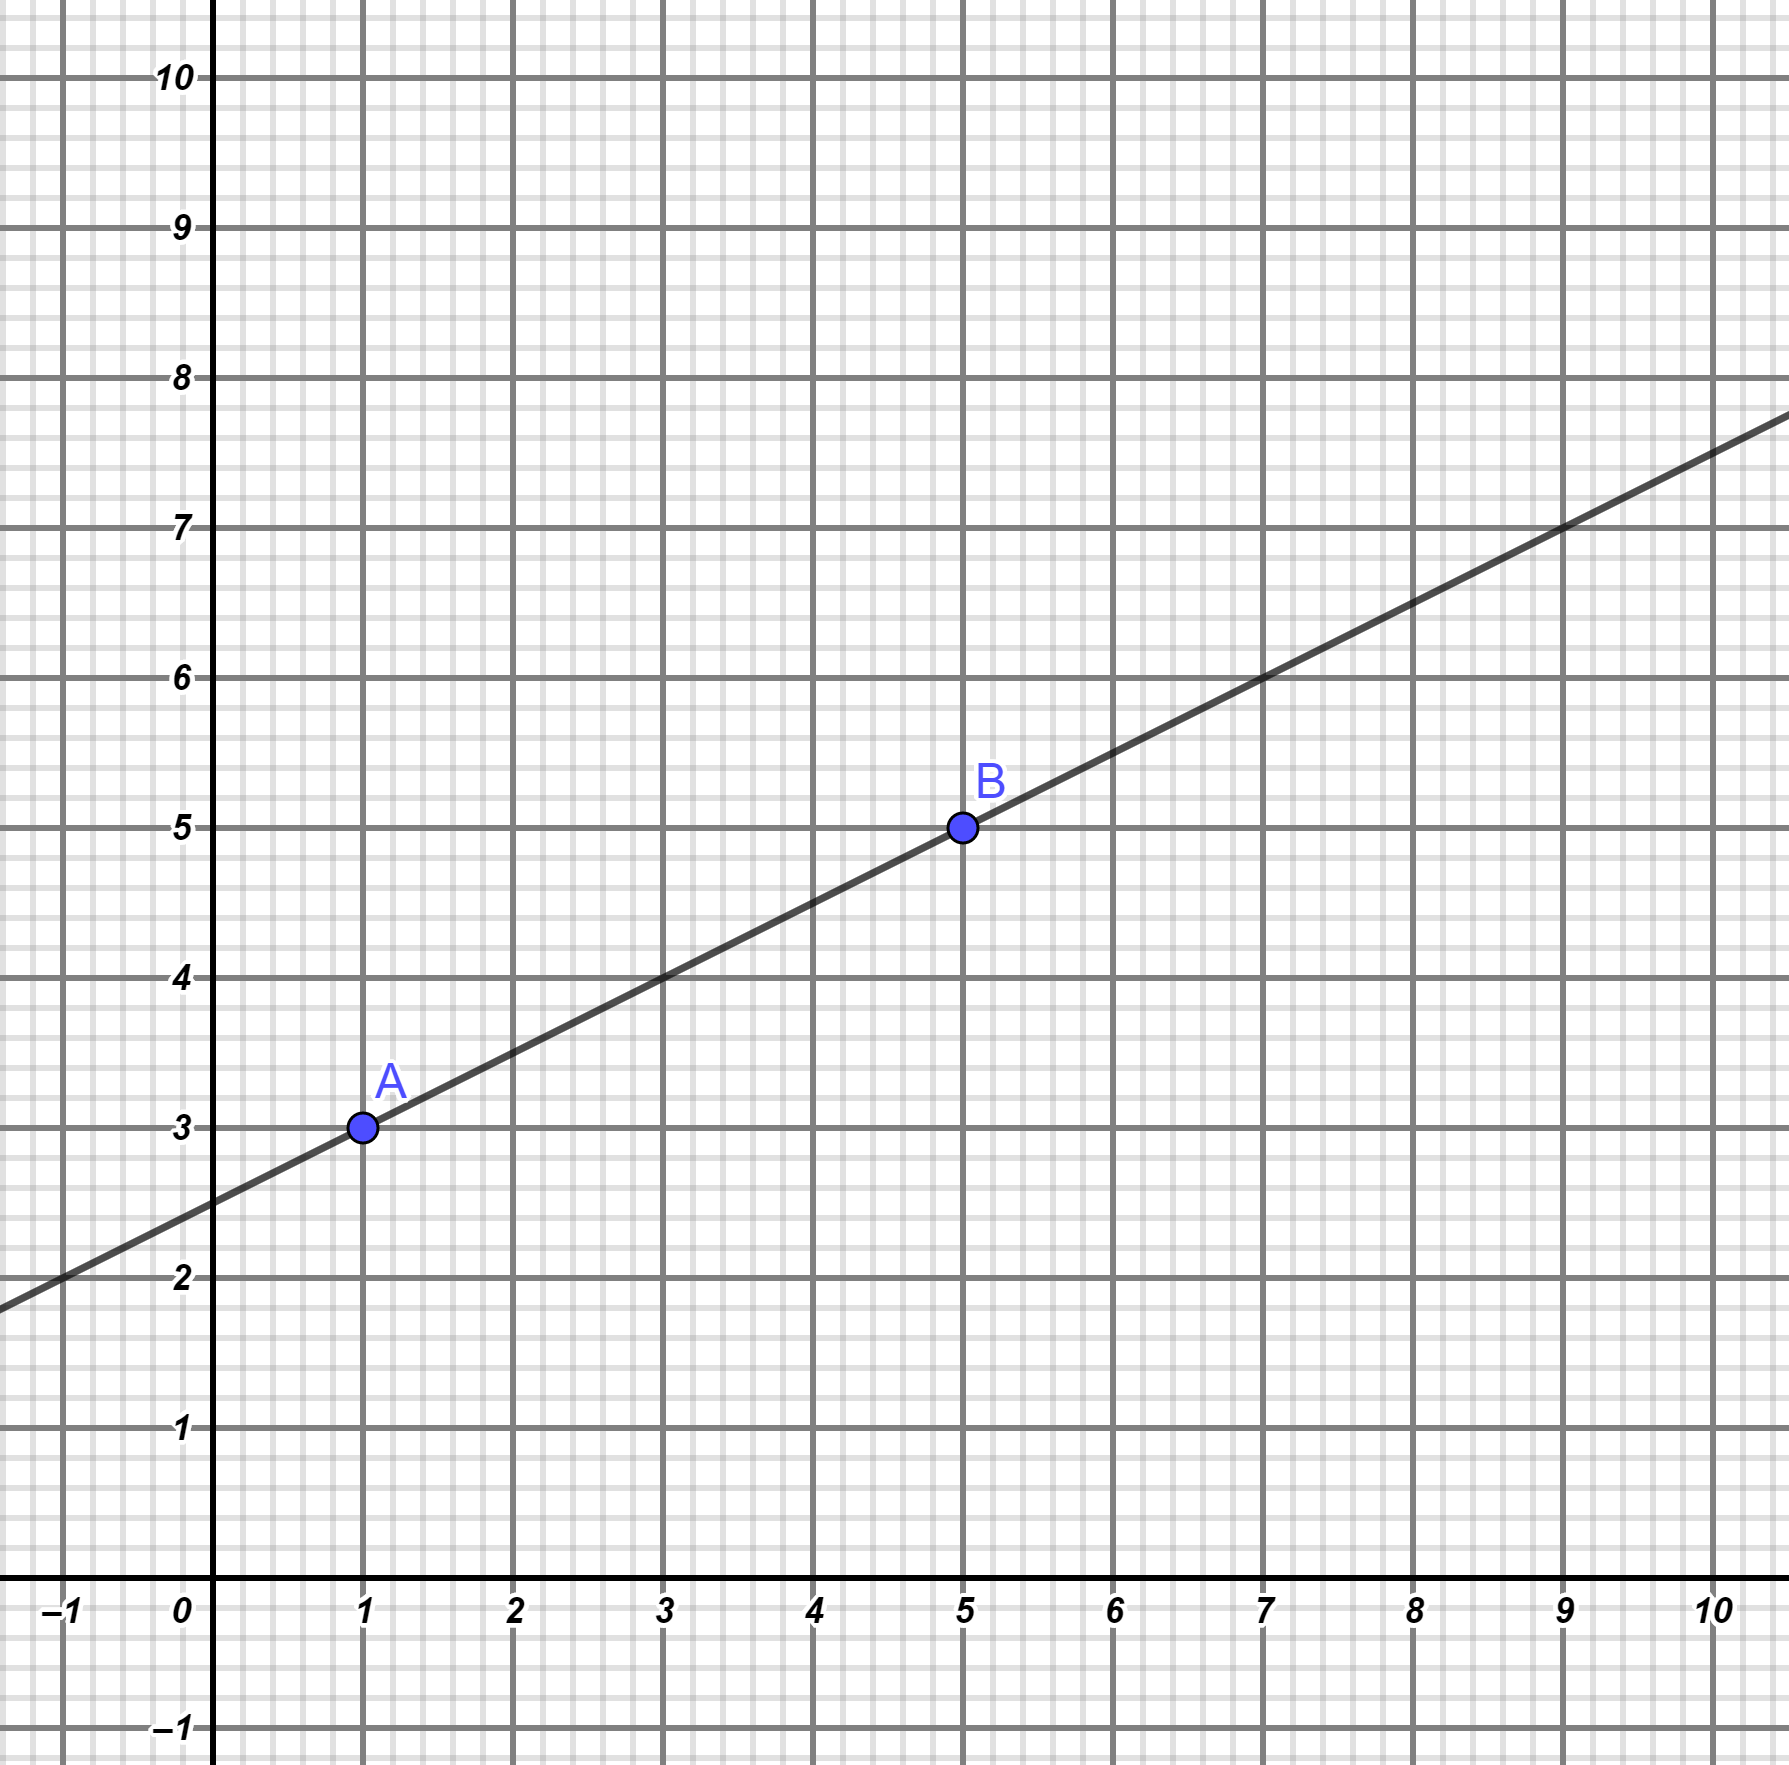
\includegraphics[scale=0.2]{img/droite2_2}
\end{center}

\begin{questions}

	
	\question[5] Déterminer l'équation de la droite $(AB)$, sous la forme $y\:=\:ax\:+\:b $.
	\fillwithdottedlines{9cm}
\end{questions}

\section{Tracer une droite}

\begin{questions}
	\question[5] Tracer dans le repère ci-dessous la droite d'équation $y\: = \: 4x \: + 2$, en détaillant le choix des points nécessaires à la construction.
	
	\begin{center}
		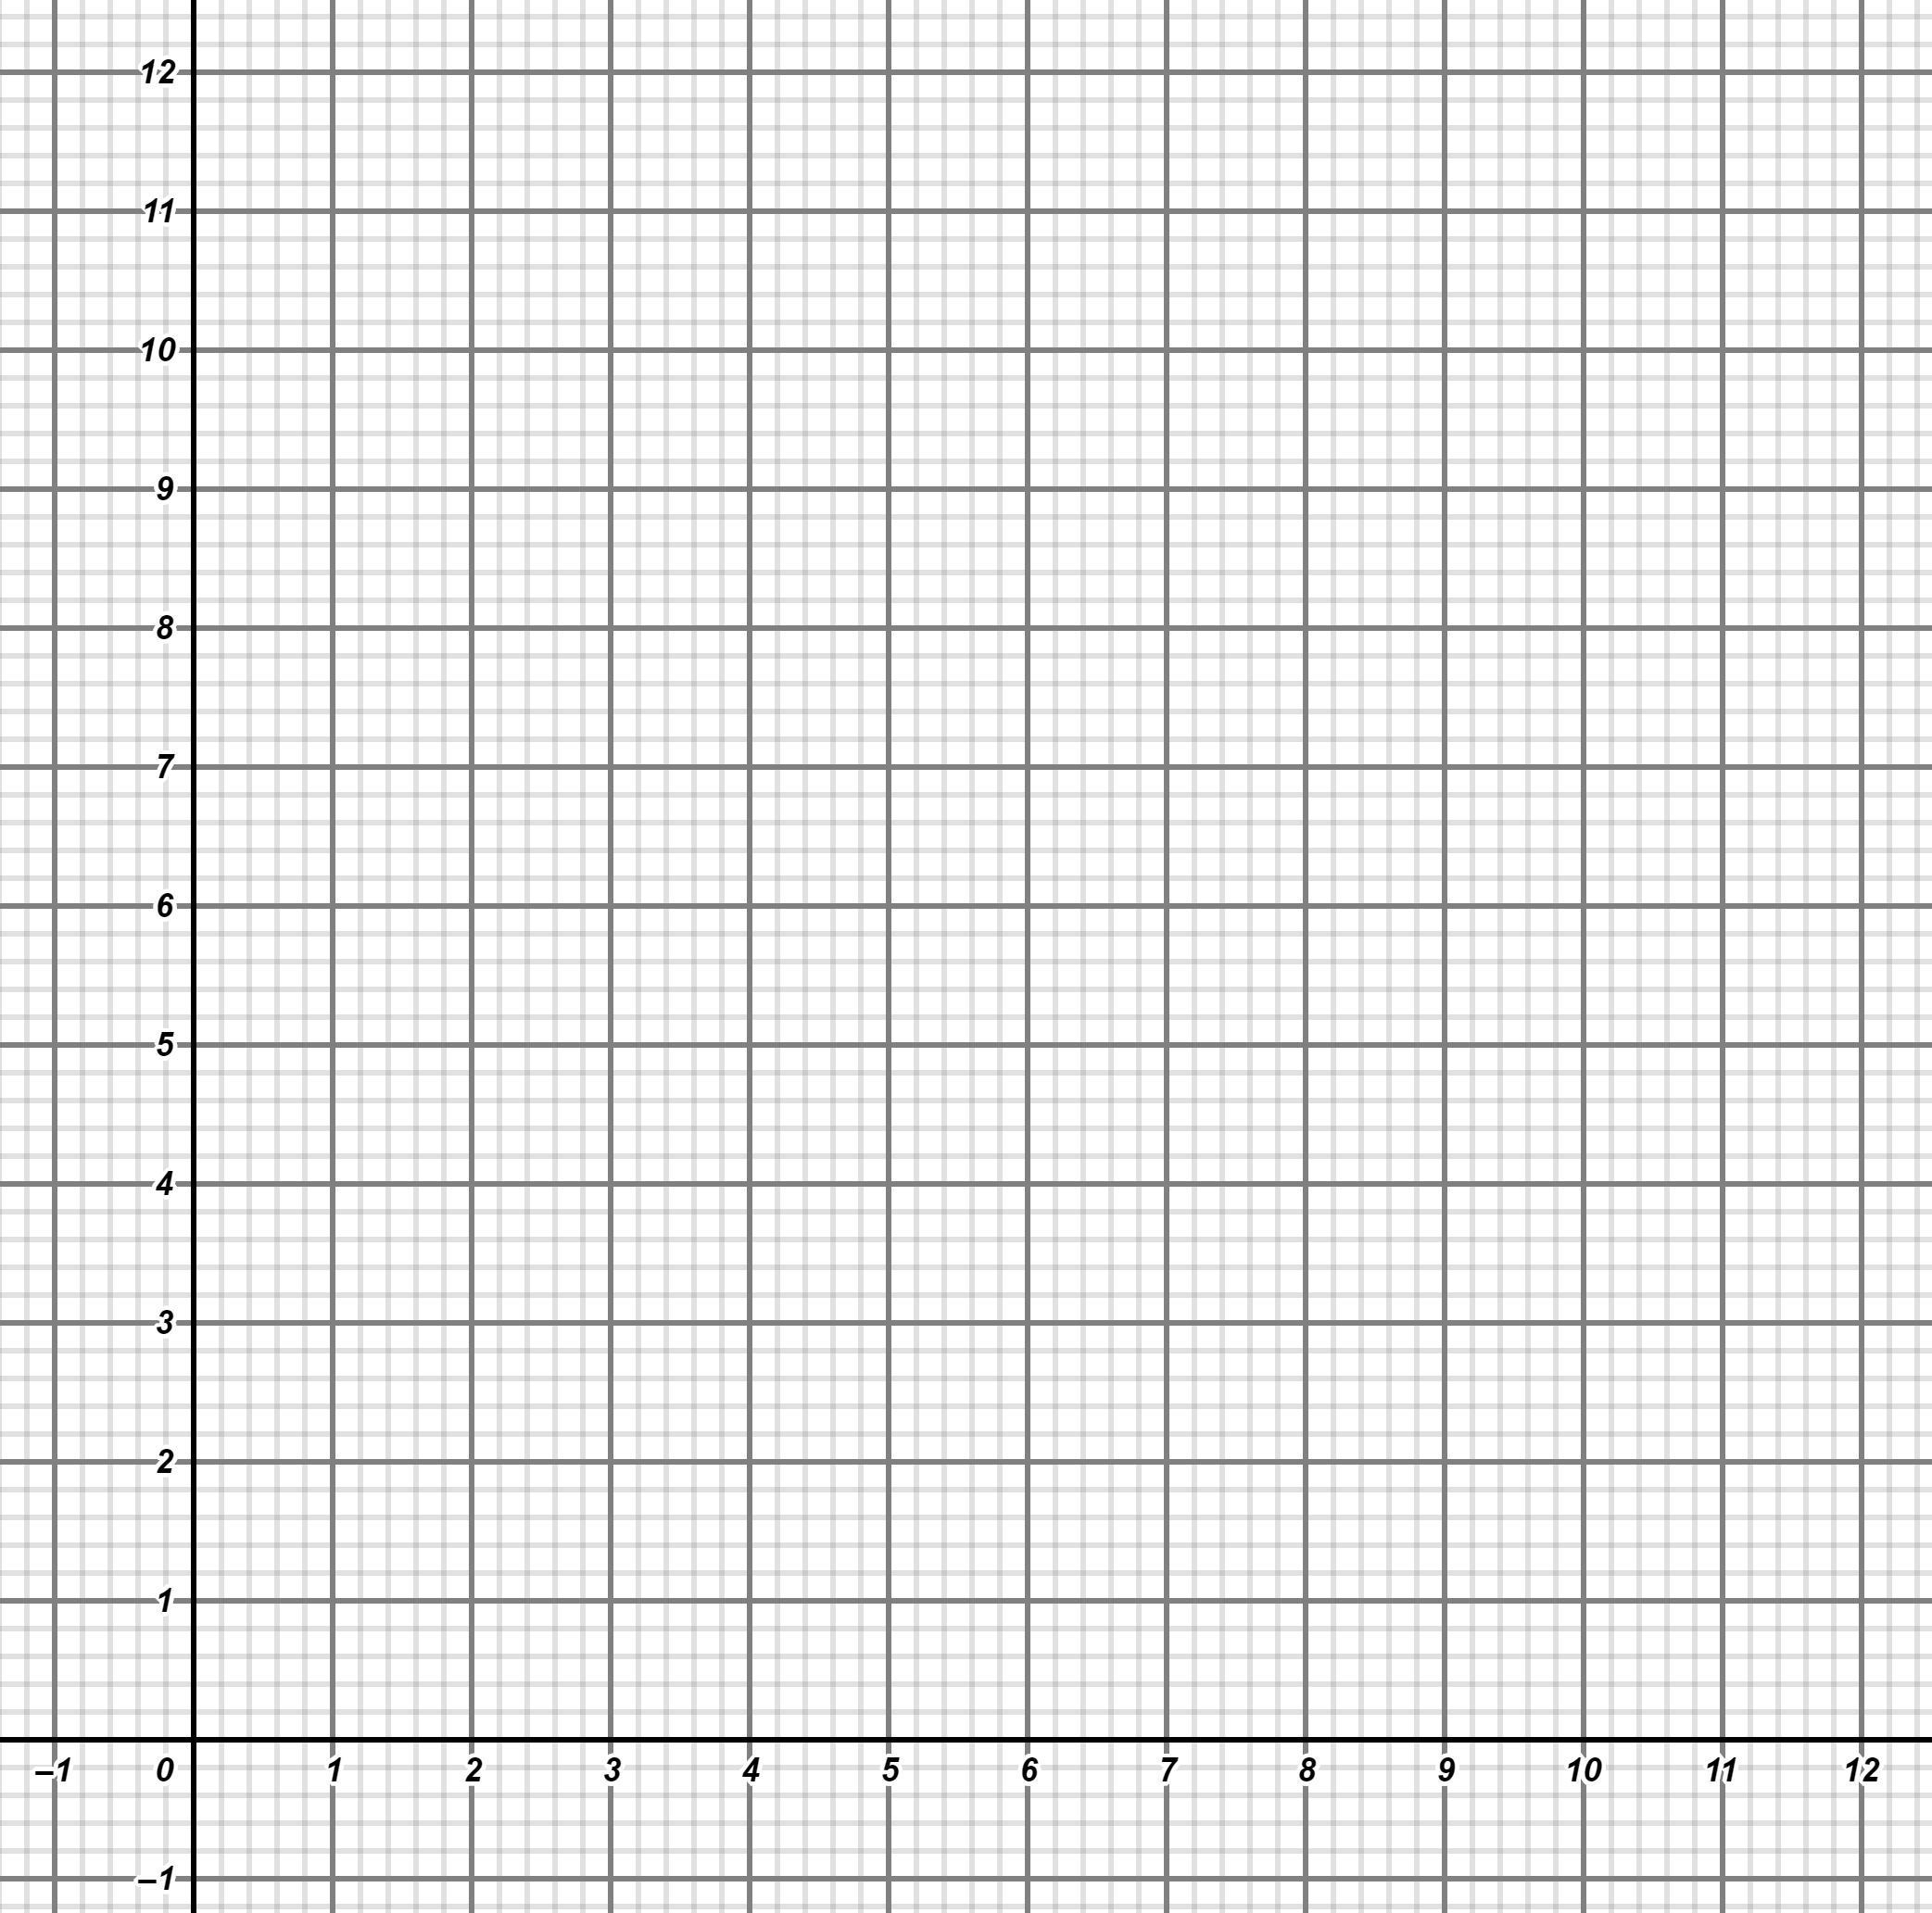
\includegraphics[scale=0.25]{img/vide_2}
	\end{center}

	\fillwithdottedlines{6cm}
\end{questions}
